

\begin{frame}
\frametitle{1. ~ Planar graphs}


A \emph{\bfseries graph} is a data structure consisting of:
\begin{itemize}[$\bullet$]
 \item A set of \emph{vertices}
 \item A set of \emph{edges} = relation between vertices
\end{itemize}


\bigskip \bigskip \pause
\begin{center}
\includegraphics[width=60pt]{images/image-78.pdf} \hspace{30pt}

\includegraphics[width=60pt]{images/image-79.pdf} \hspace{30pt}

\includegraphics[width=60pt]{images/image-80.pdf}
\end{center}

\bigskip \bigskip
\pause
{\bfseries Applications of graph theory:} 
Computer science (networks), linguistics, physics and chemistry, biology, social sciences, \etc{}


\end{frame}



\begin{frame}
\frametitle{1. ~ Planar graphs}


\bigskip

A graph is called \emph{\bfseries planar} if it can be drawn on the plane with no edge crossings.

\medskip \pause
\begin{center}

\includegraphics[width=60pt]{images/image-115.pdf} \hspace{30pt}
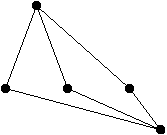
\includegraphics[width=70pt]{images/image-116.pdf}
\end{center}

\medskip \pause
\begin{center}
\includegraphics[width=55pt]{images/image-118-tetra.pdf} \hspace{20pt}

\includegraphics[width=40pt]{images/image-117.pdf} \hspace{20pt}

\includegraphics[width=55pt]{images/image-118.pdf} \hspace{20pt}

\includegraphics[width=55pt]{images/image-118-tetra2.pdf}
\end{center}

\medskip \pause
\begin{center}

\includegraphics[width=50pt]{images/image-124.pdf} \hspace{30pt} \pause
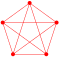
\includegraphics[width=60pt]{images/image-122-red.pdf}
\end{center}


\end{frame}
